% Plot the various performance indicators to illustrate the team choice and various result in data preprocessing & mining
\section{Data Visualization}\label{data_visualisation}

This section encompasses the graphical representation of data features and model architectures for enhanced comprehension.

\begin{description}[style=nextline]
    \item[Feature Visualization:] Visual depiction of both given and derived features for enhanced understanding.
    \item[Convolution Neural Network:] Visual representation of CNN model architecture to facilitate interpretation.
    \item[Multilayer Perceptron:] Visual depiction of MLP model architecture for improved insight into its workings.
\end{description}

\subsection{Feature Visualization}\label{feature_visualization}

\subsubsection{Frequency Graph of LOS and NLOS}\label{frequency_graph}

\begin{figure}[H] 
	\centering
	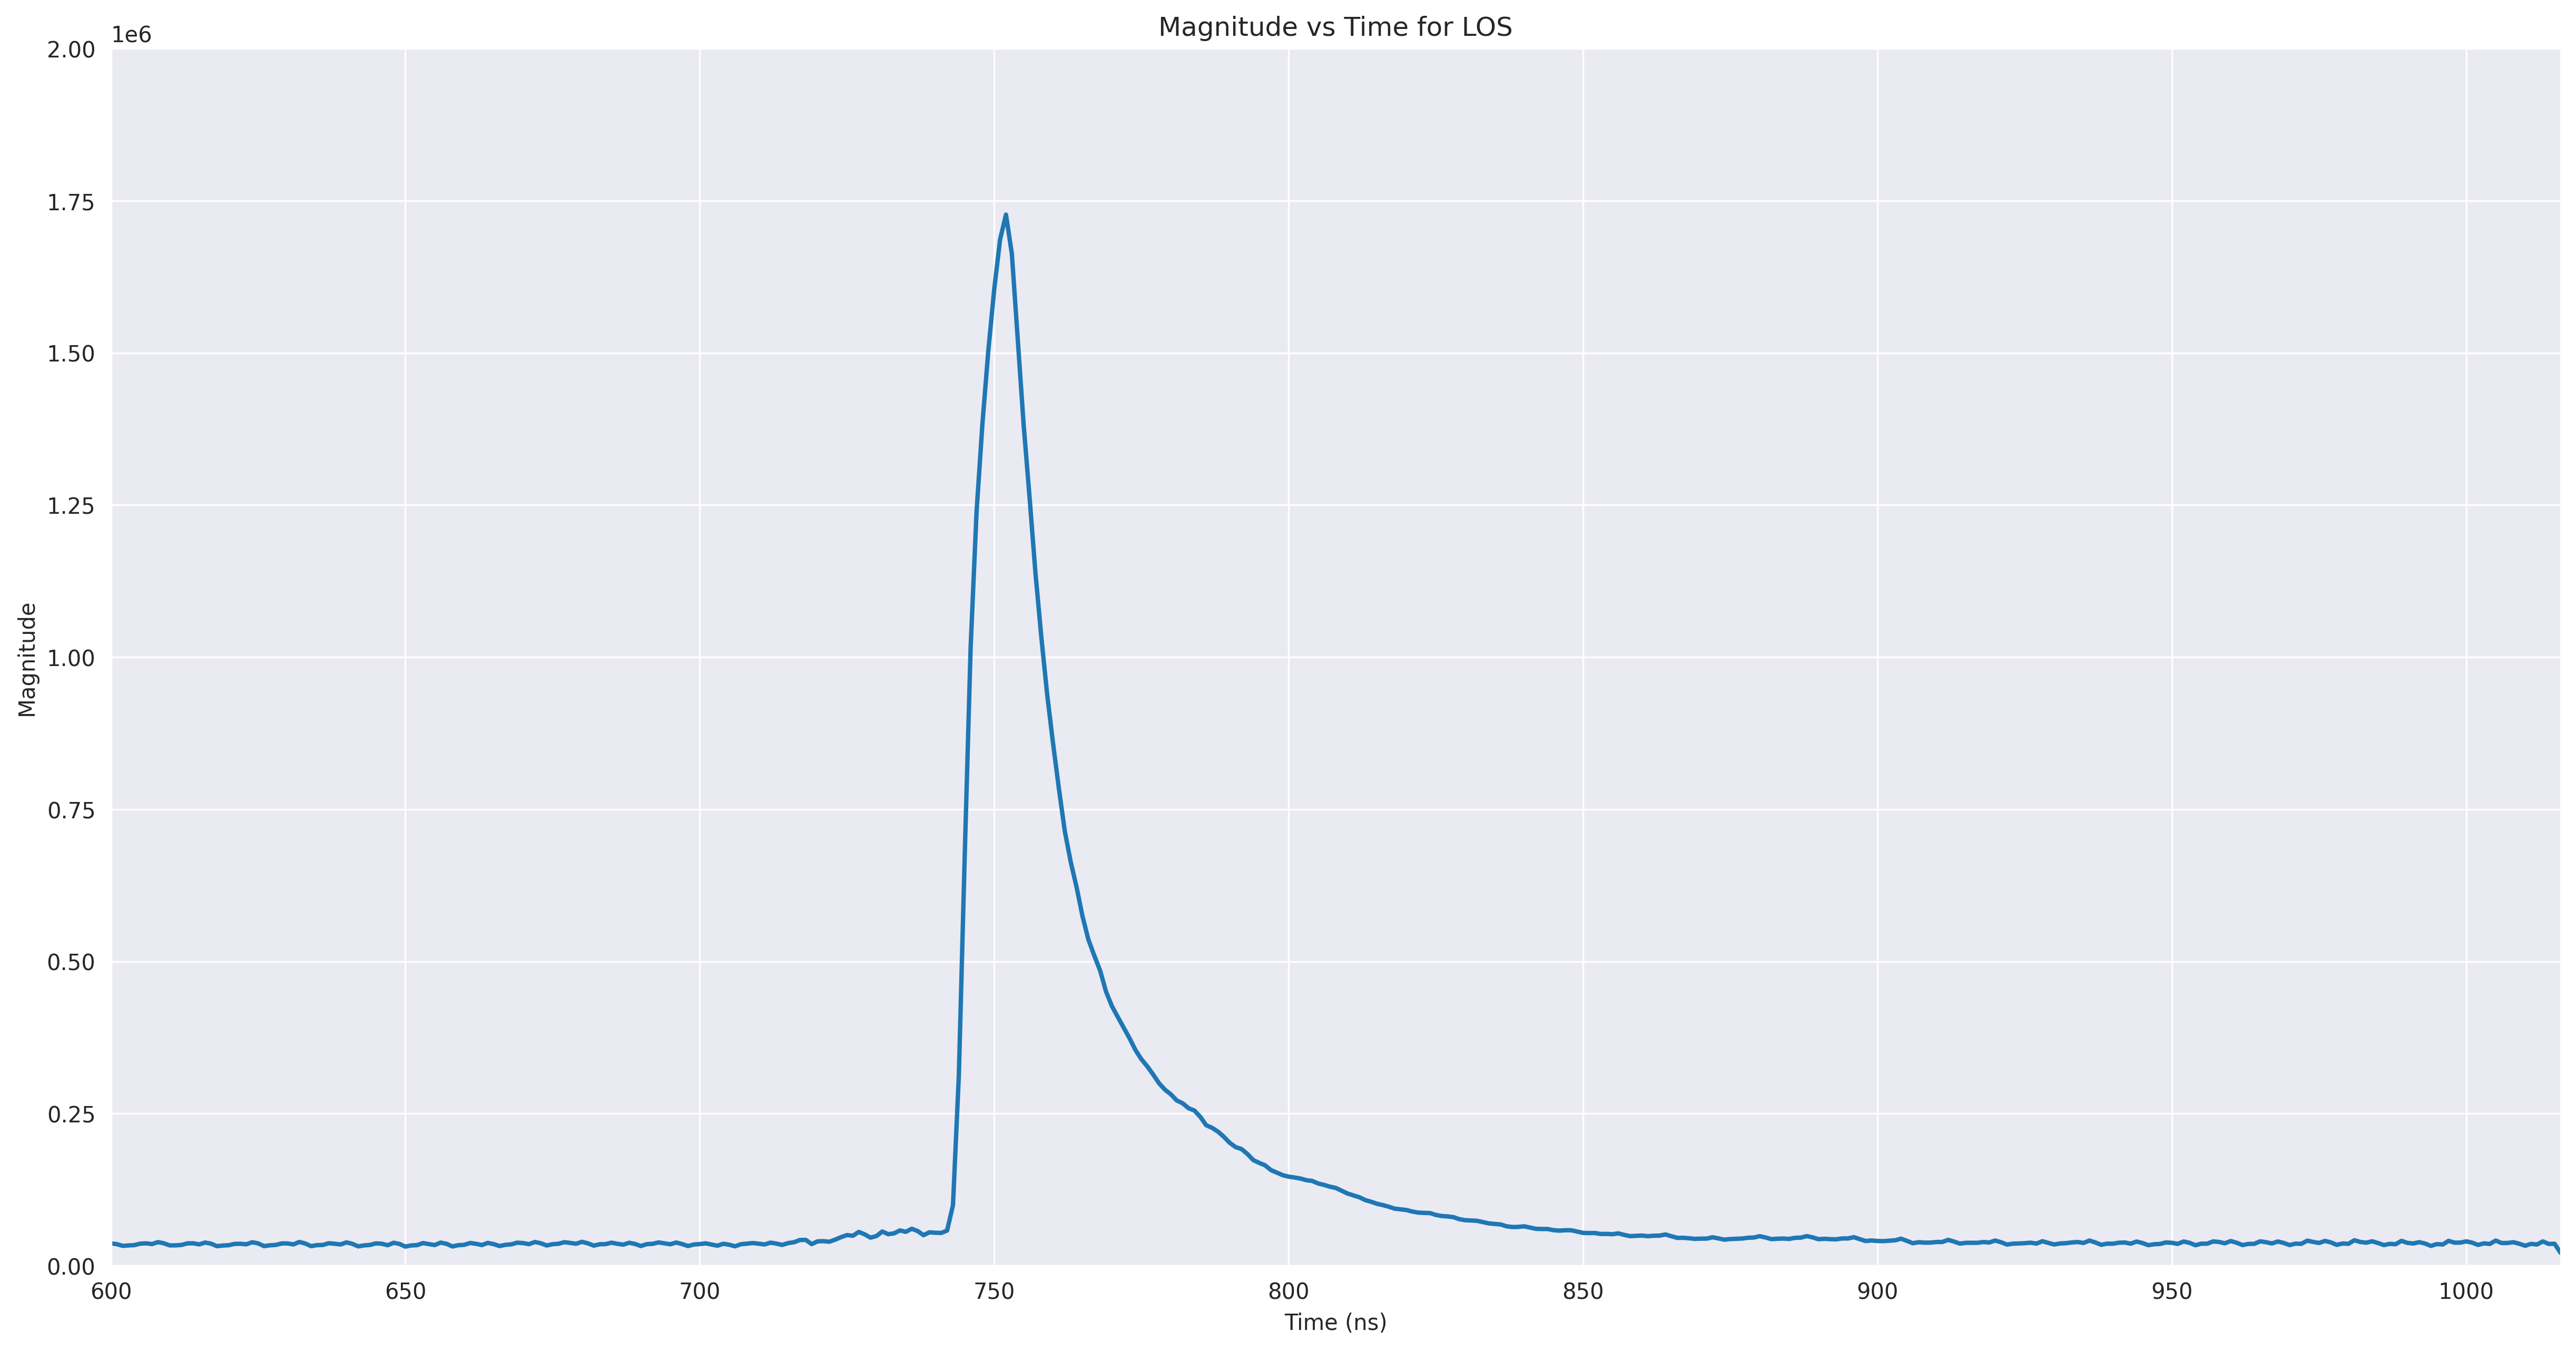
\includegraphics[width=1\textwidth]{preprocessing/LOS_Frequency_Graph.png}
	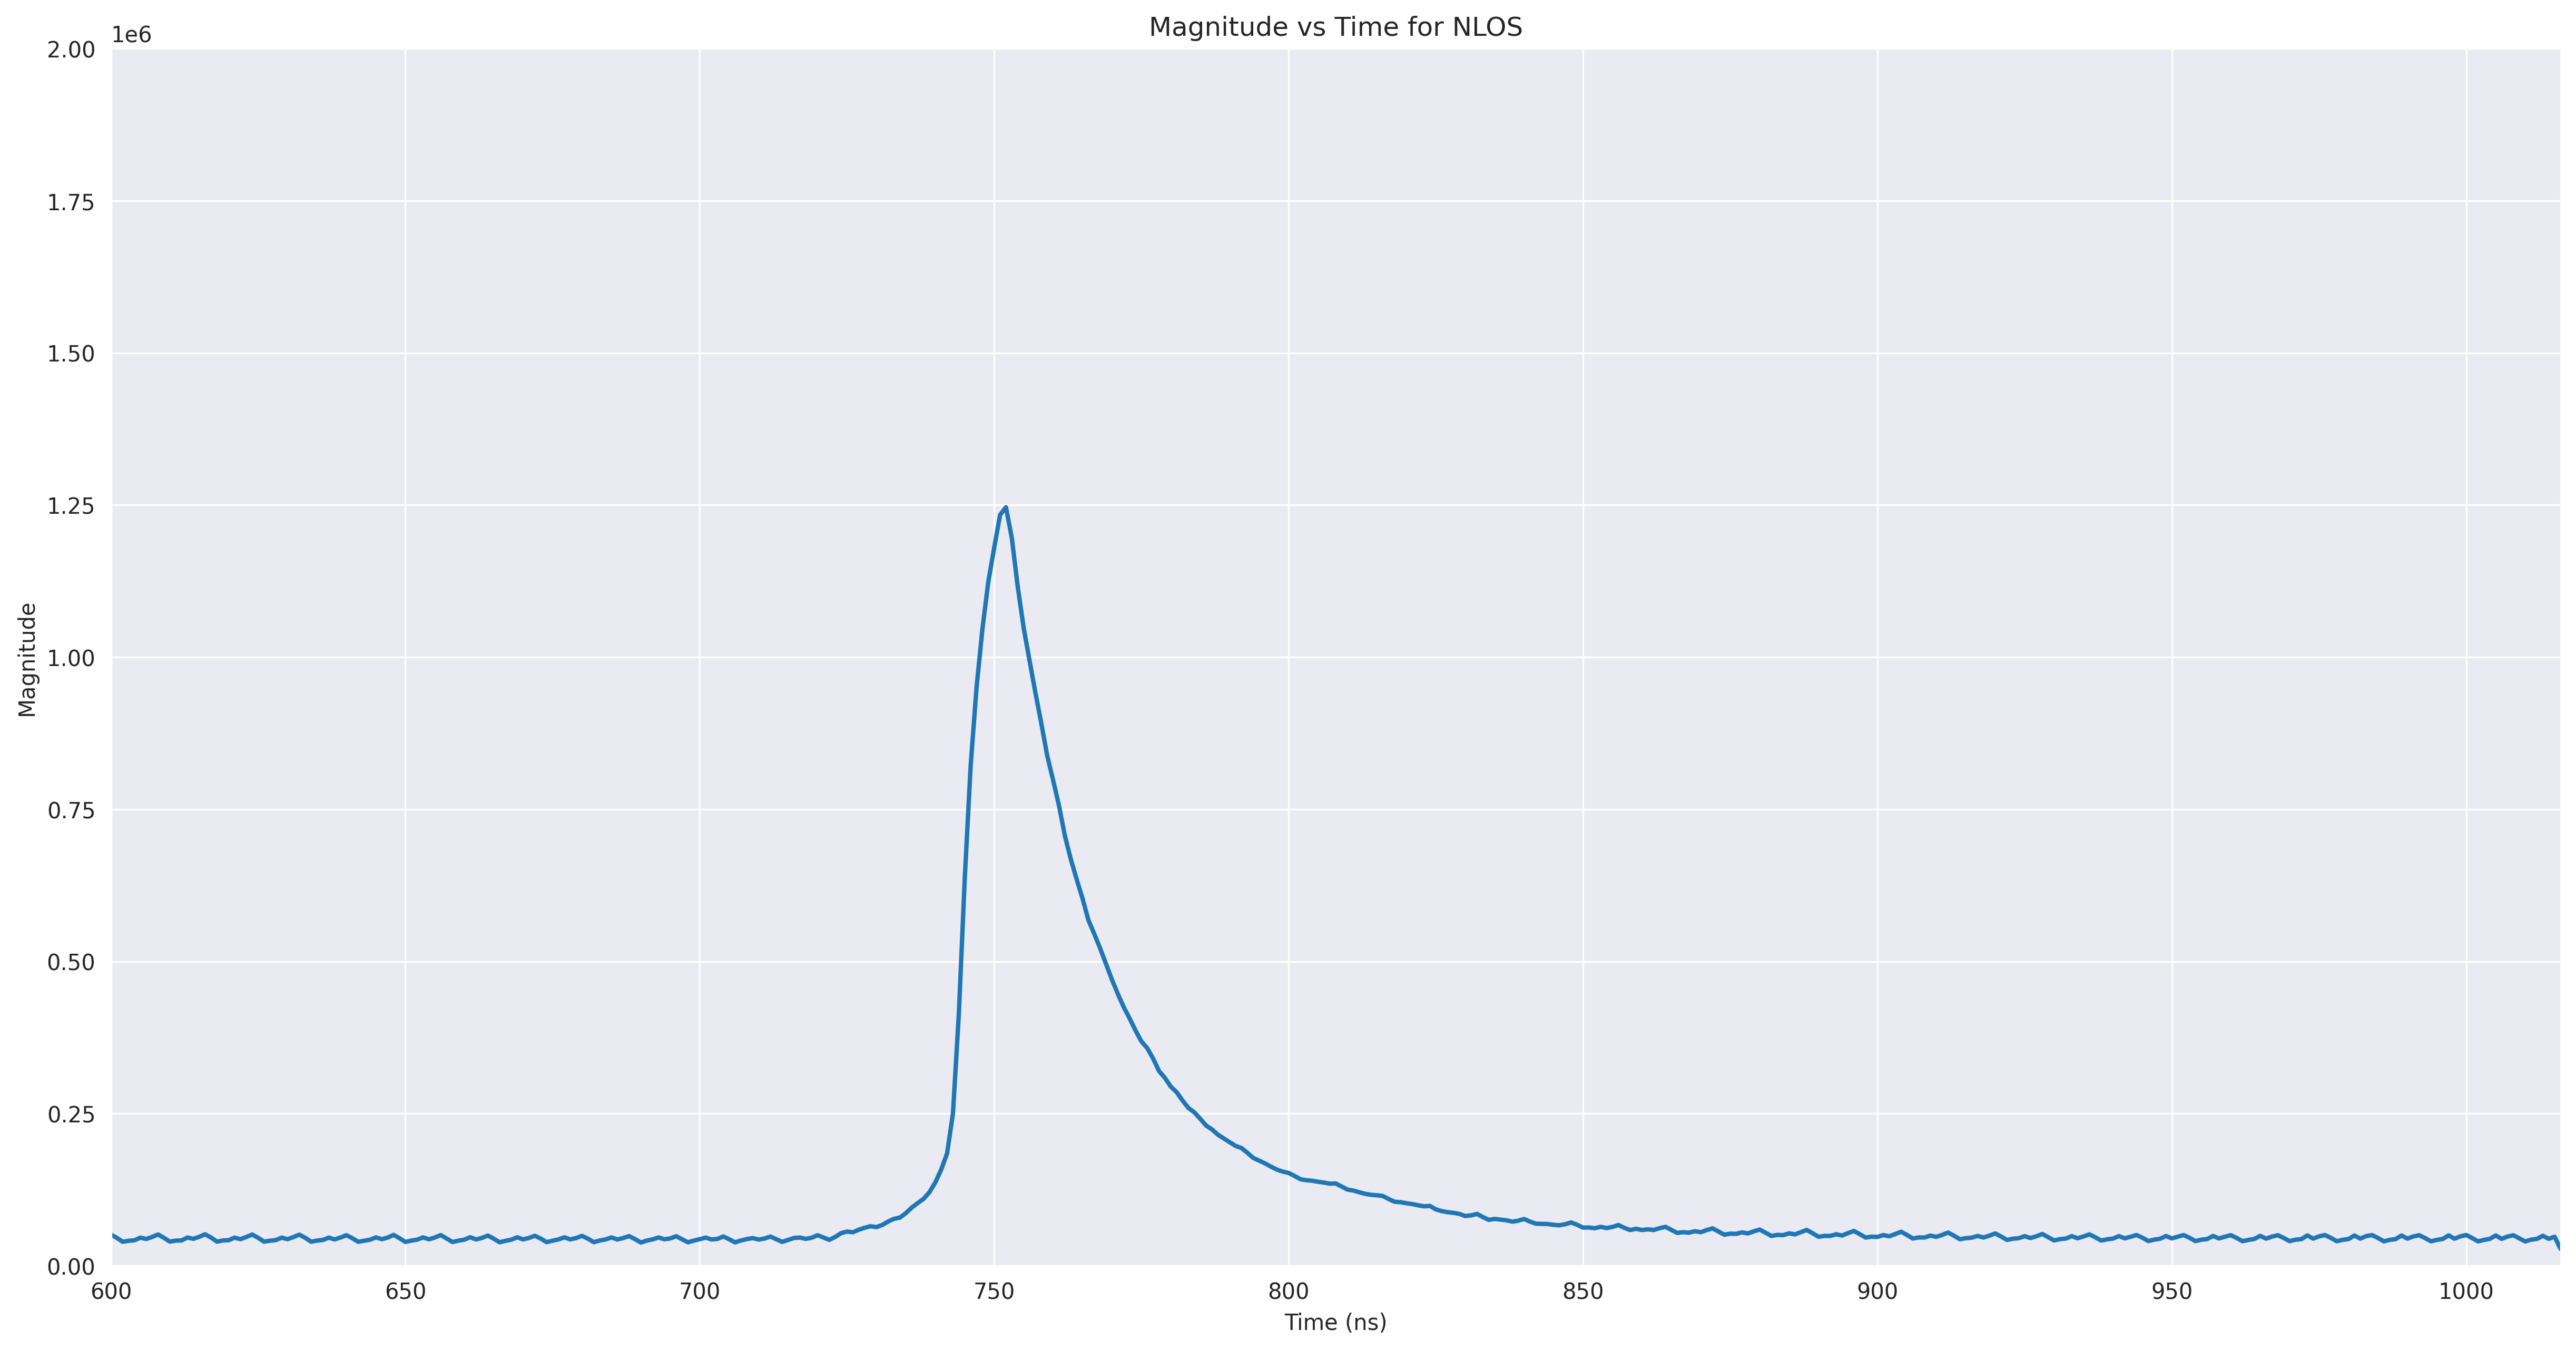
\includegraphics[width=1\textwidth]{preprocessing/NLOS_Frequency_Graph.png}
	\caption{Frequency Graph of LOS and NLOS}\label{fig:frequency_graph}
\end{figure}

\subsubsection{Frequency Graph of Wavelet Transformed LOS and NLOS}\label{frequency_graph_wavelet}

\begin{figure}[H] 
  \centering
  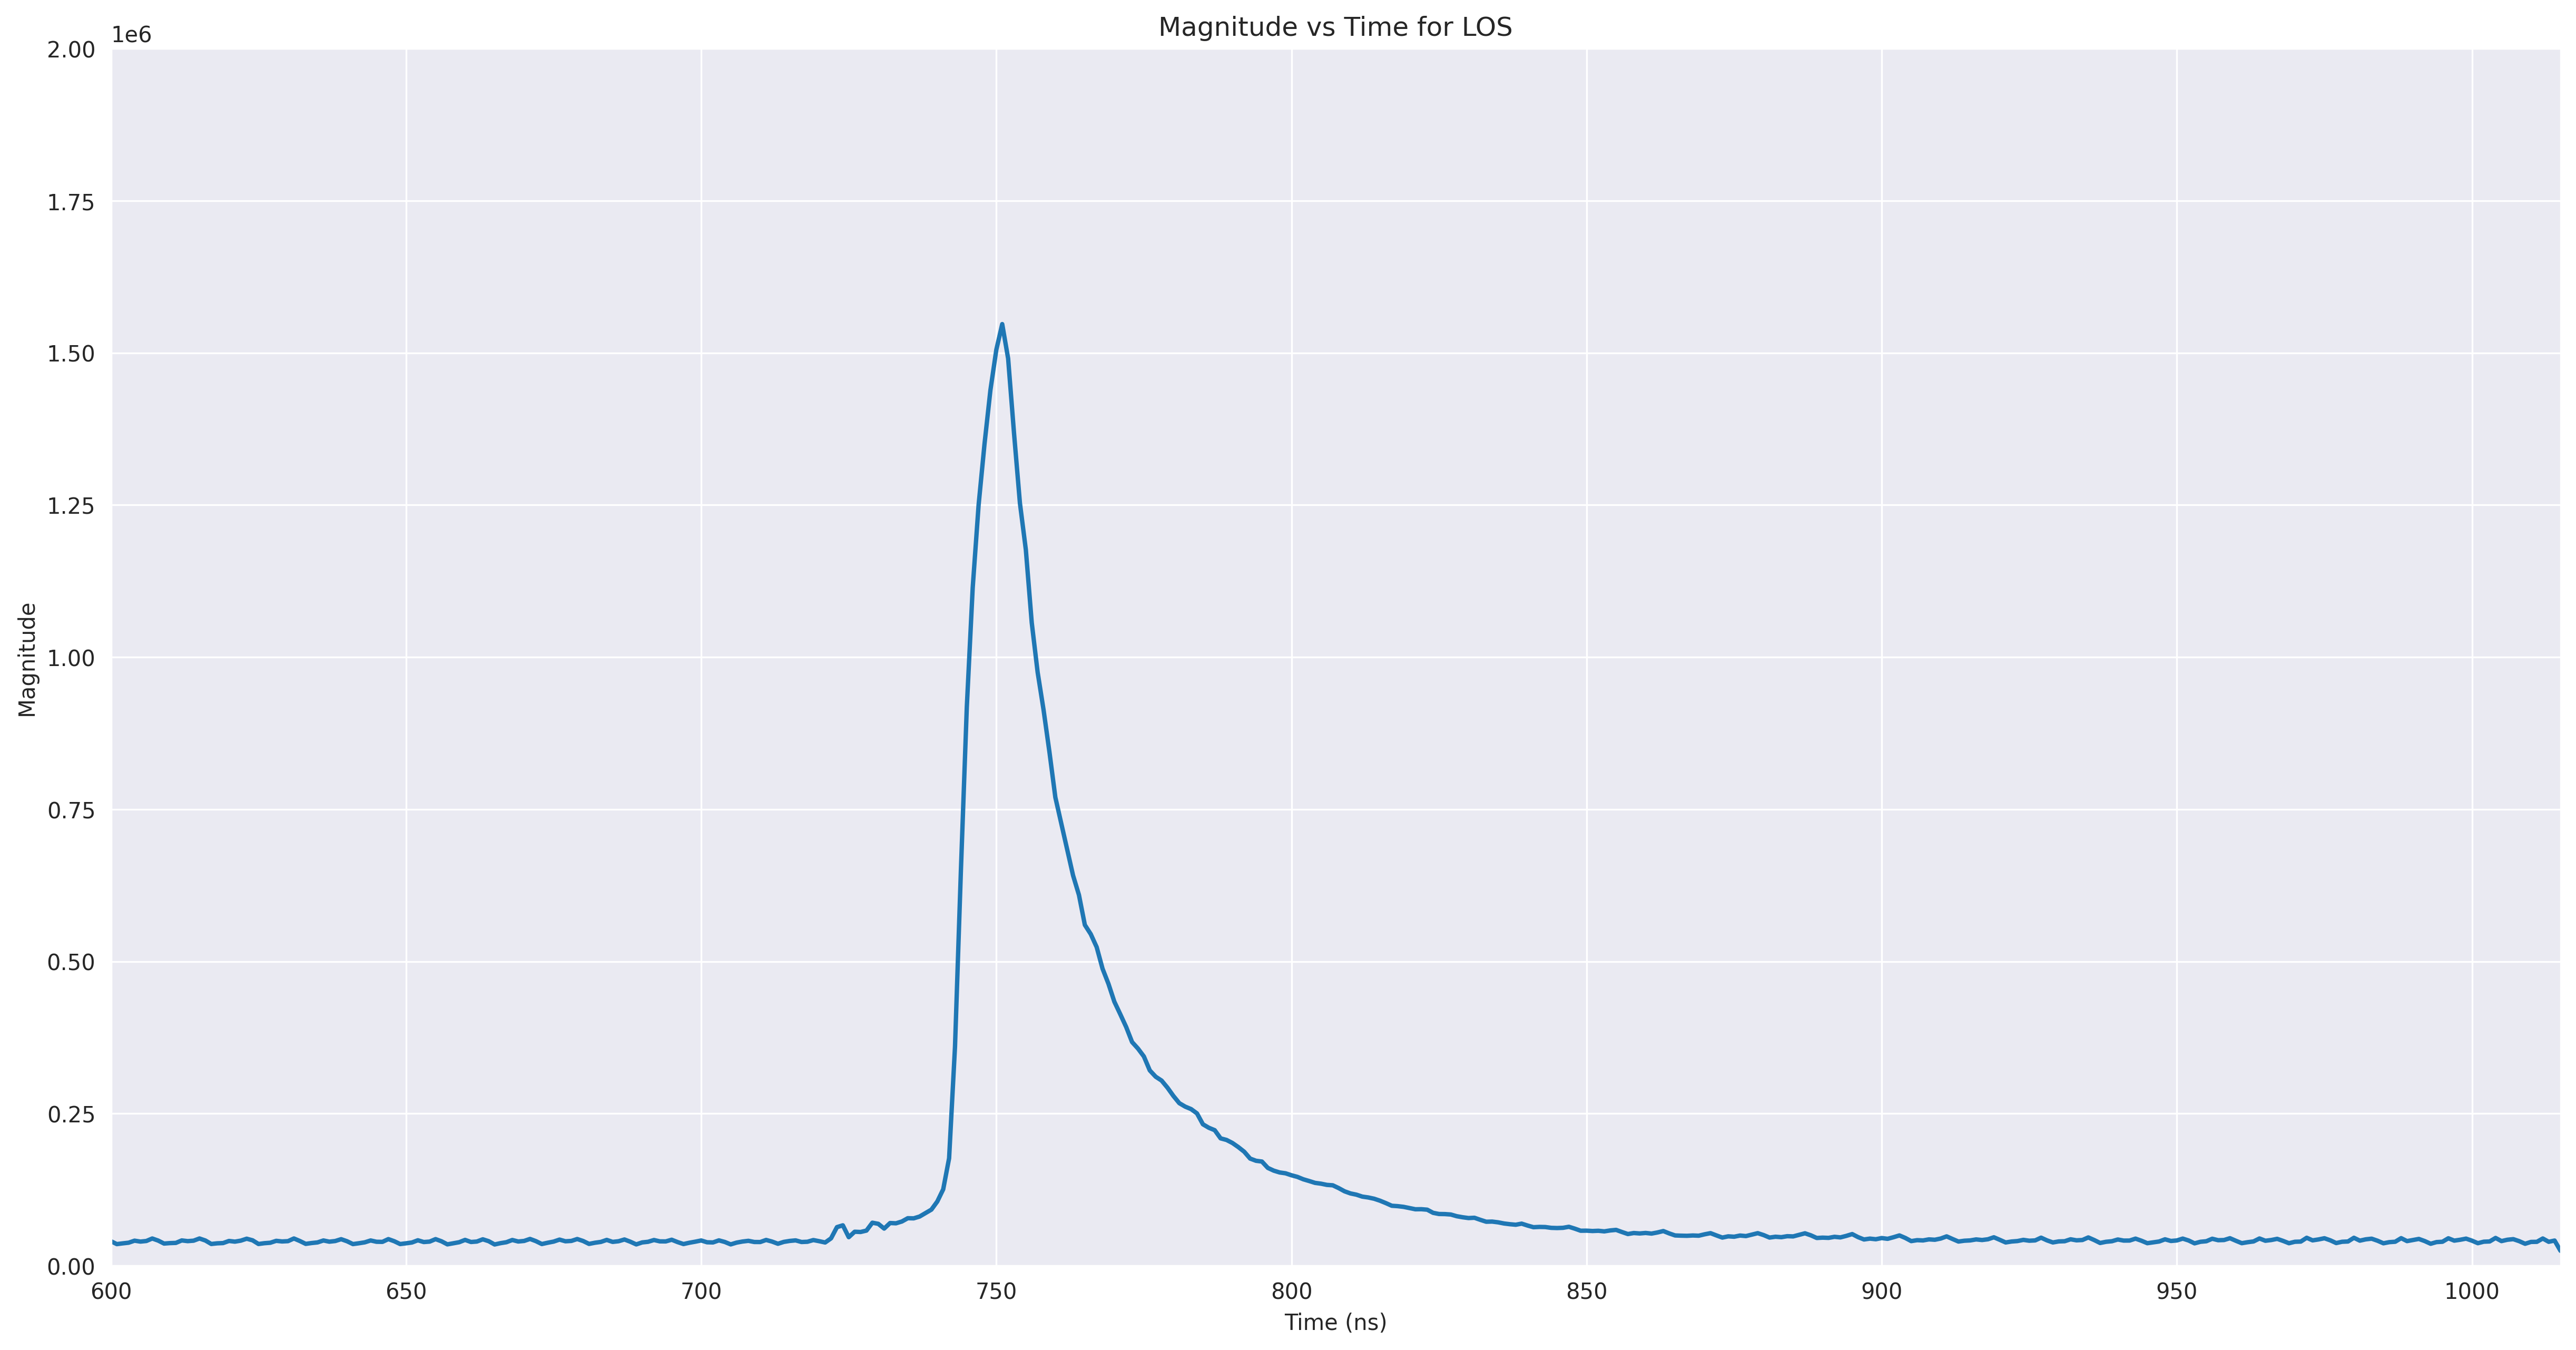
\includegraphics[width=1\textwidth]{preprocessing/Wavelet_Denoised_LOS_Frequency_Graph.png}
  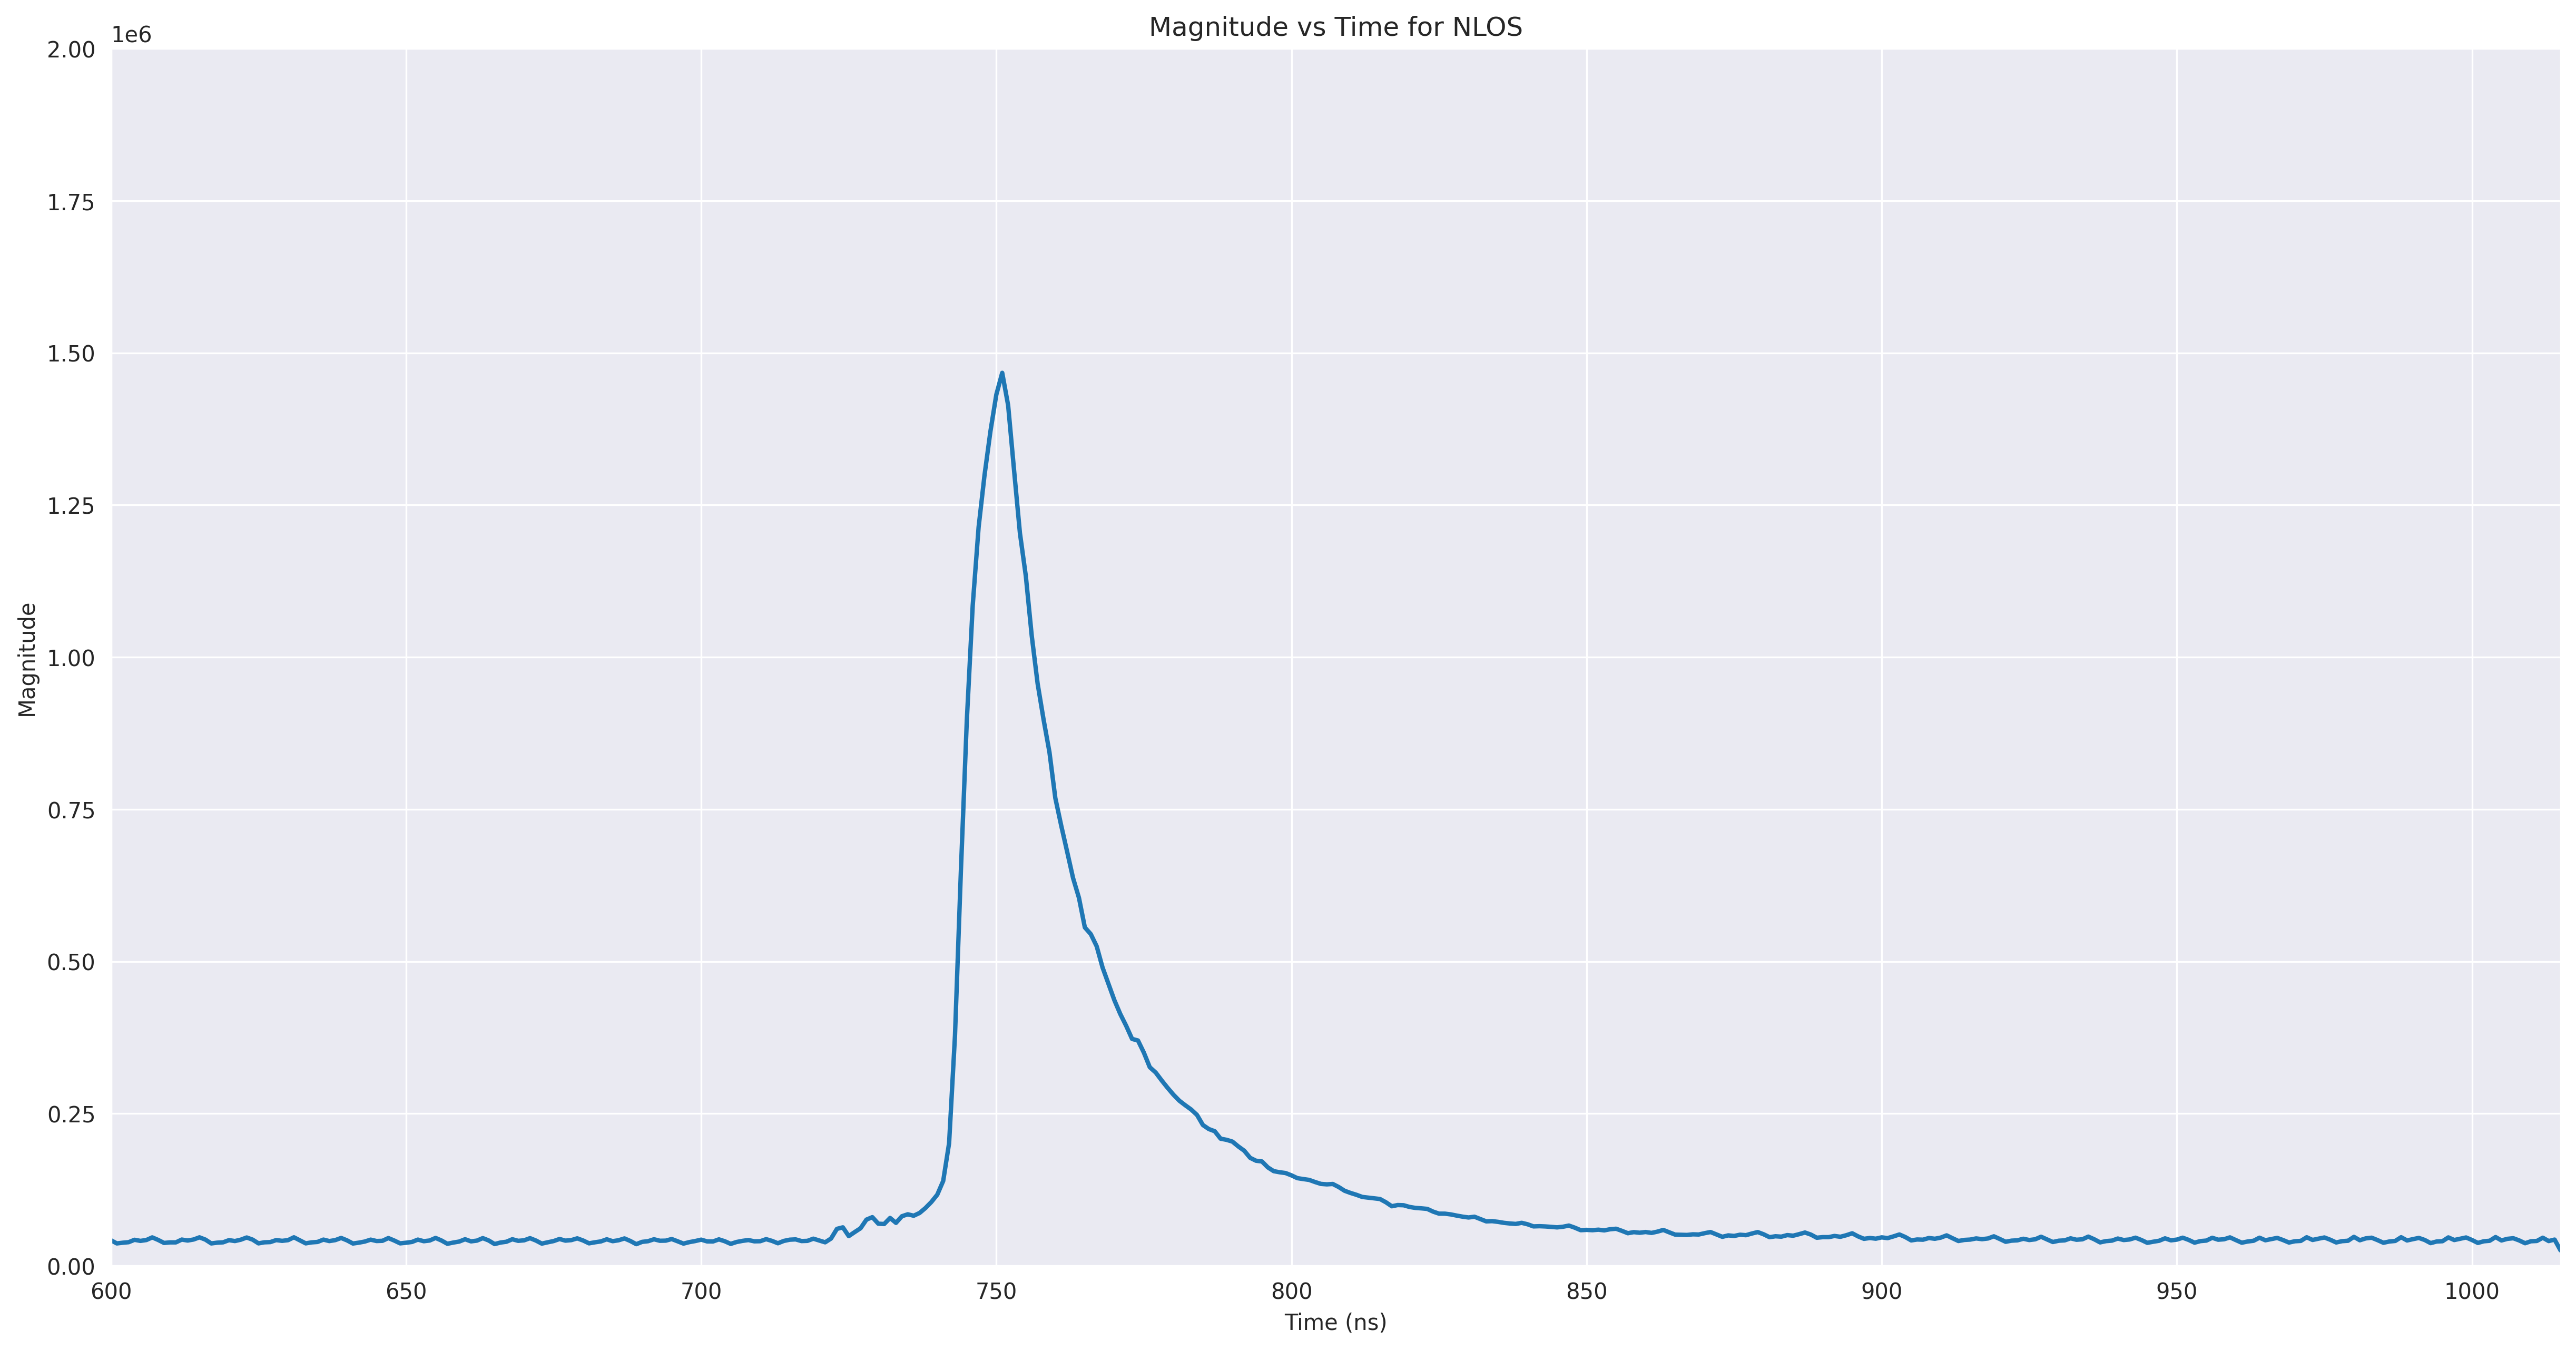
\includegraphics[width=1\textwidth]{preprocessing/Wavelet_Denoised_NLOS_Frequency_Graph.png}
  \caption{Frequency Graph of Wavelet Transformed LOS and NLOS}\label{fig:frequency_graph_wavelet}
\end{figure}

\subsubsection{Frequency Graph of Lucy-Richardson Transformation LOS and NLOS}\label{frequency_graph_lr}

\begin{figure}[H] 
  \centering
  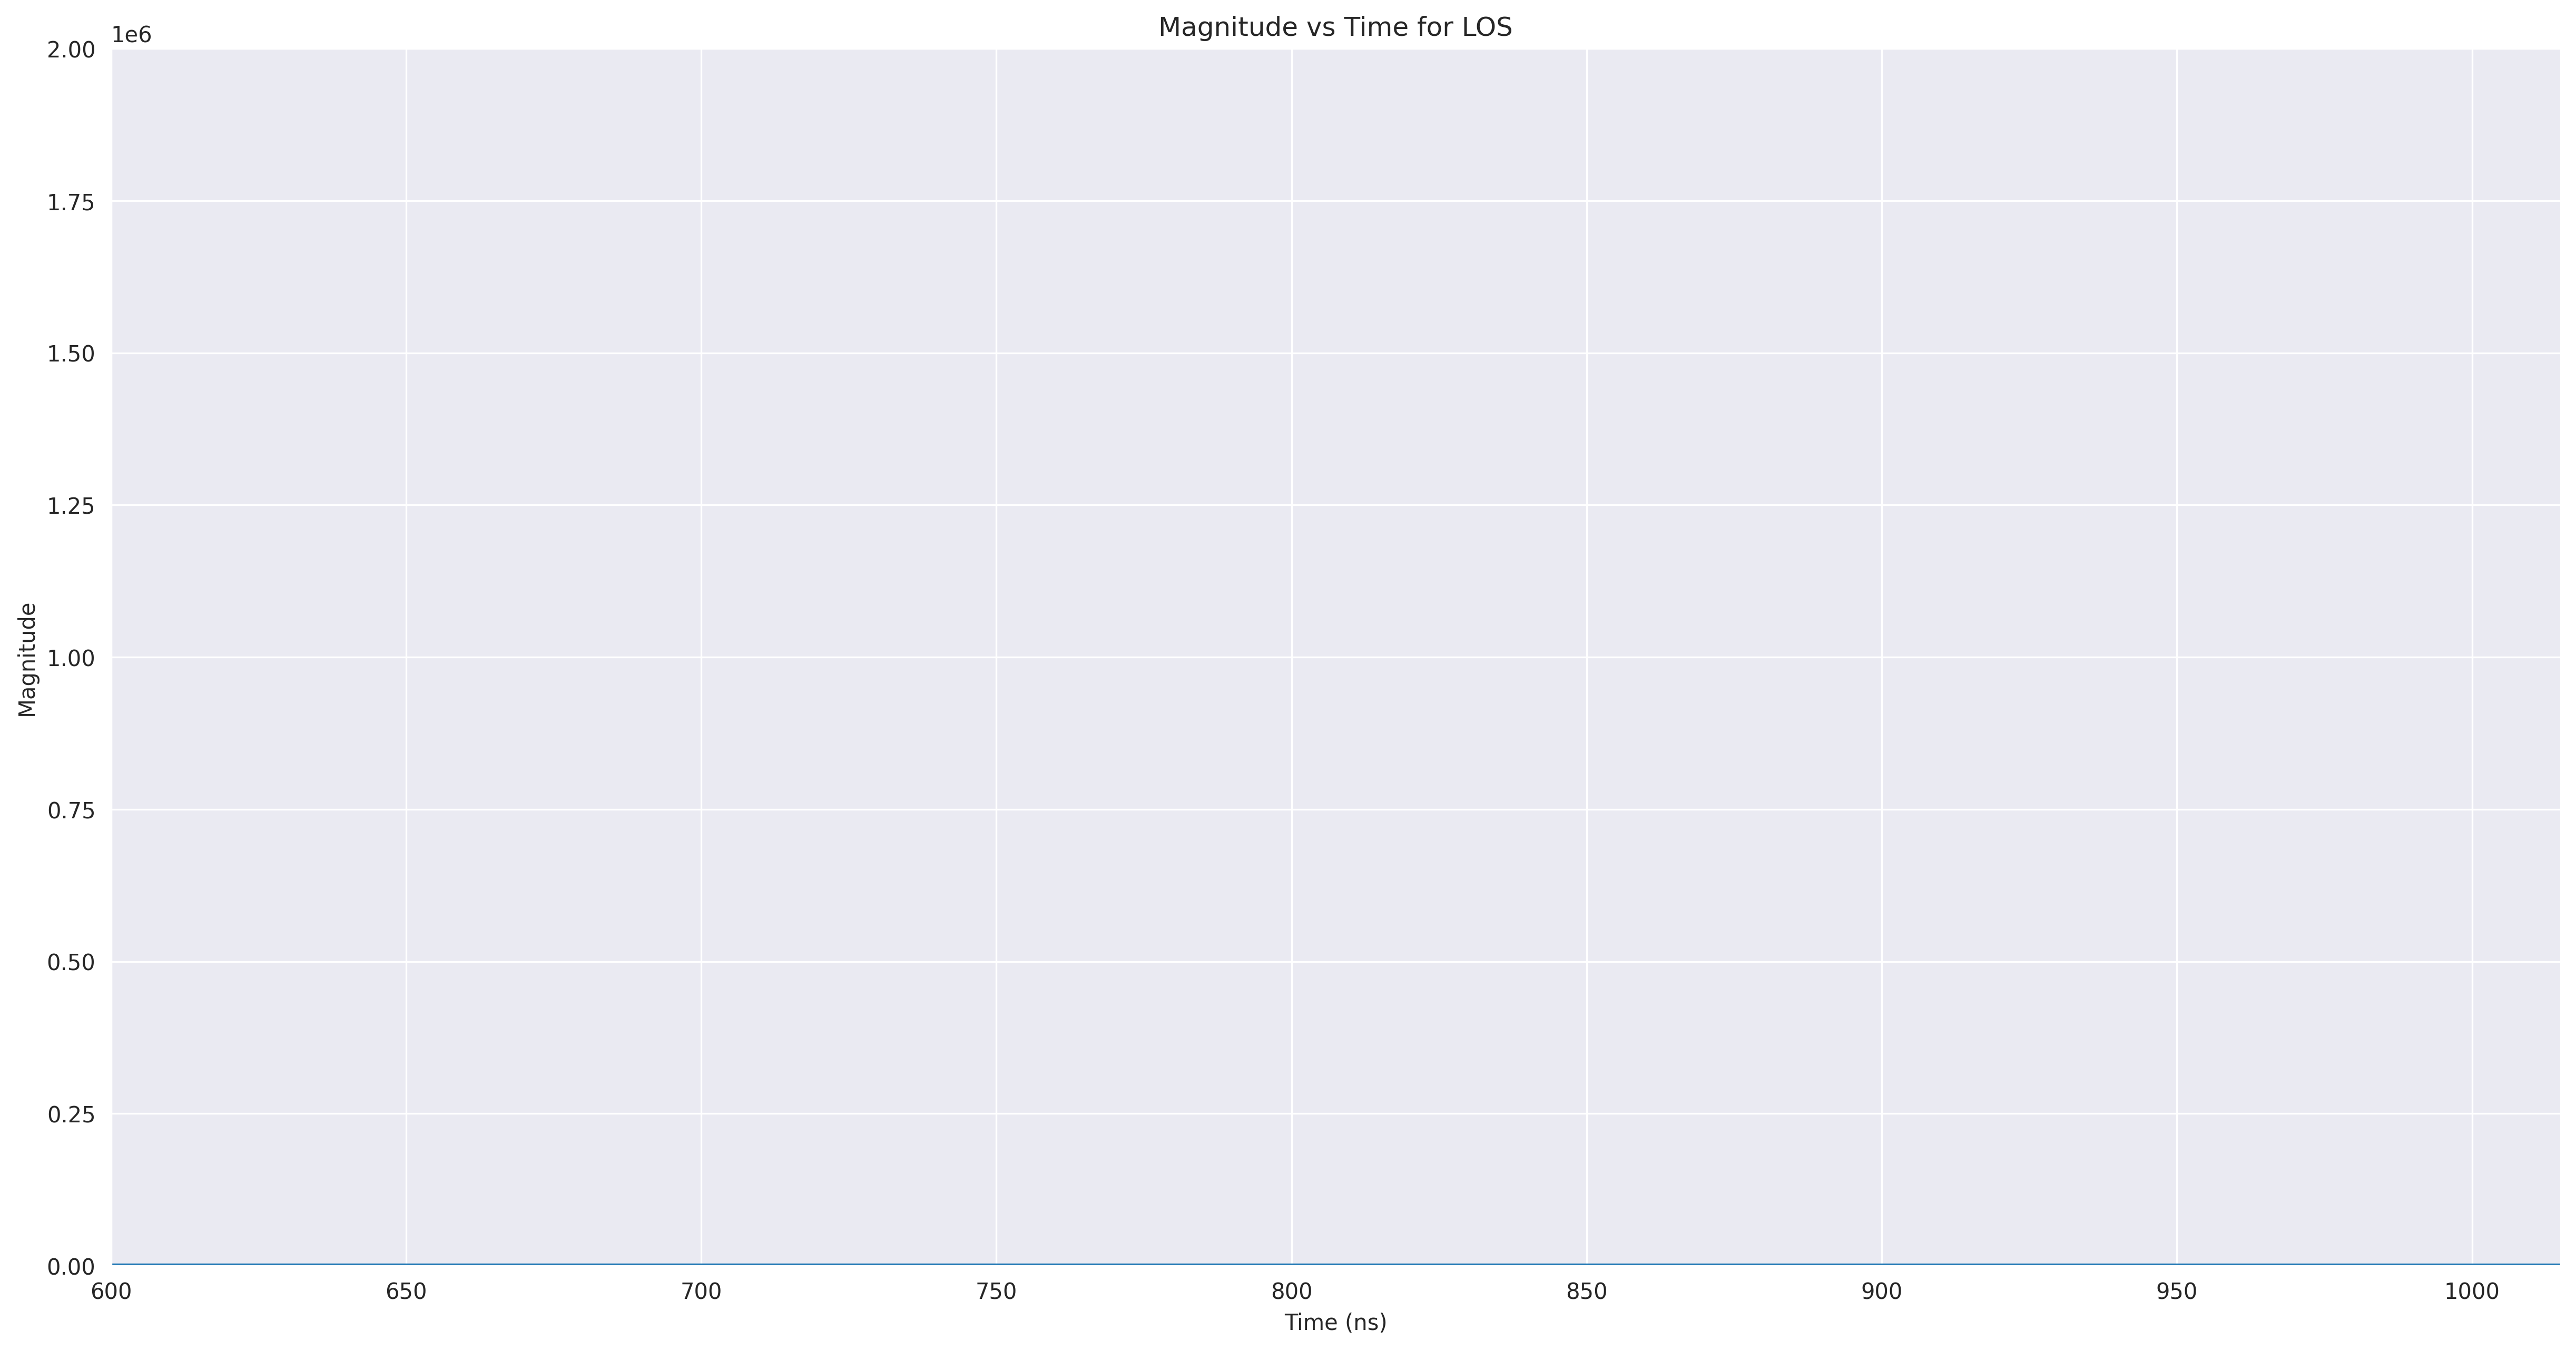
\includegraphics[width=1\textwidth]{preprocessing/lr_denoise_LOS.png}
  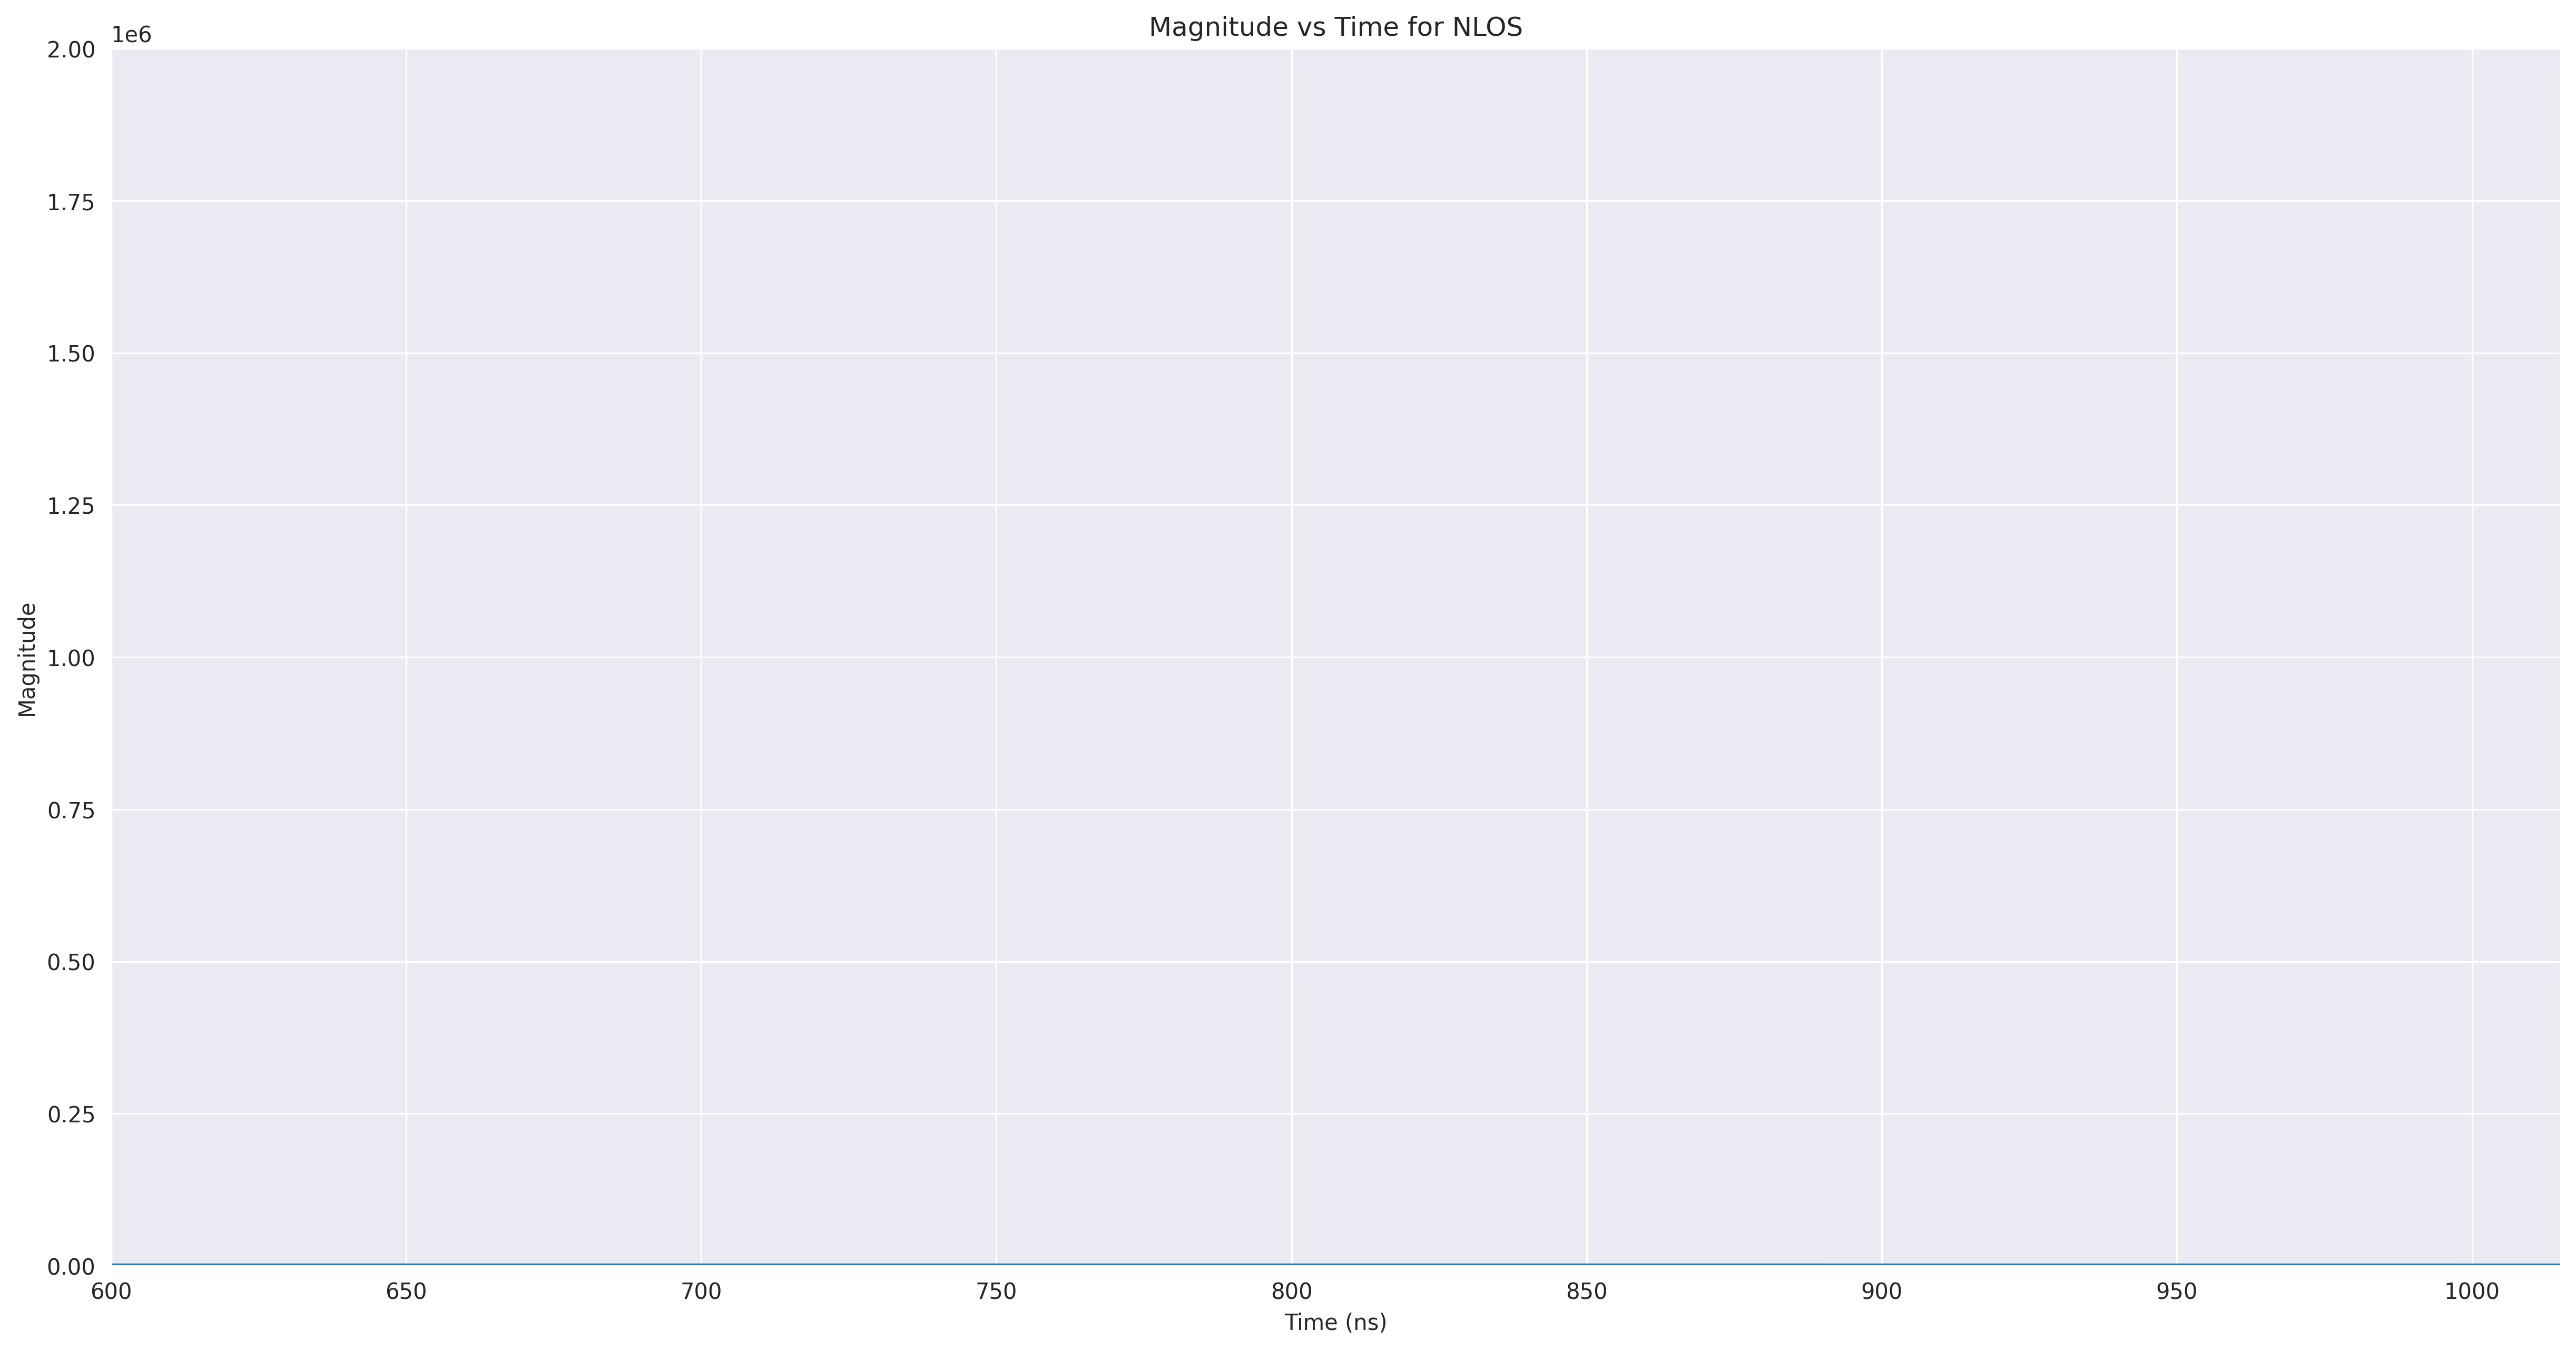
\includegraphics[width=1\textwidth]{preprocessing/lr_denoise_NLOS.png}
  \caption{Frequency Graph of Lucy-Richardson(Unscaled) LOS and NLOS}\label{fig:frequency_graph_lr}
\end{figure}

\begin{figure}[H] 
  \centering
  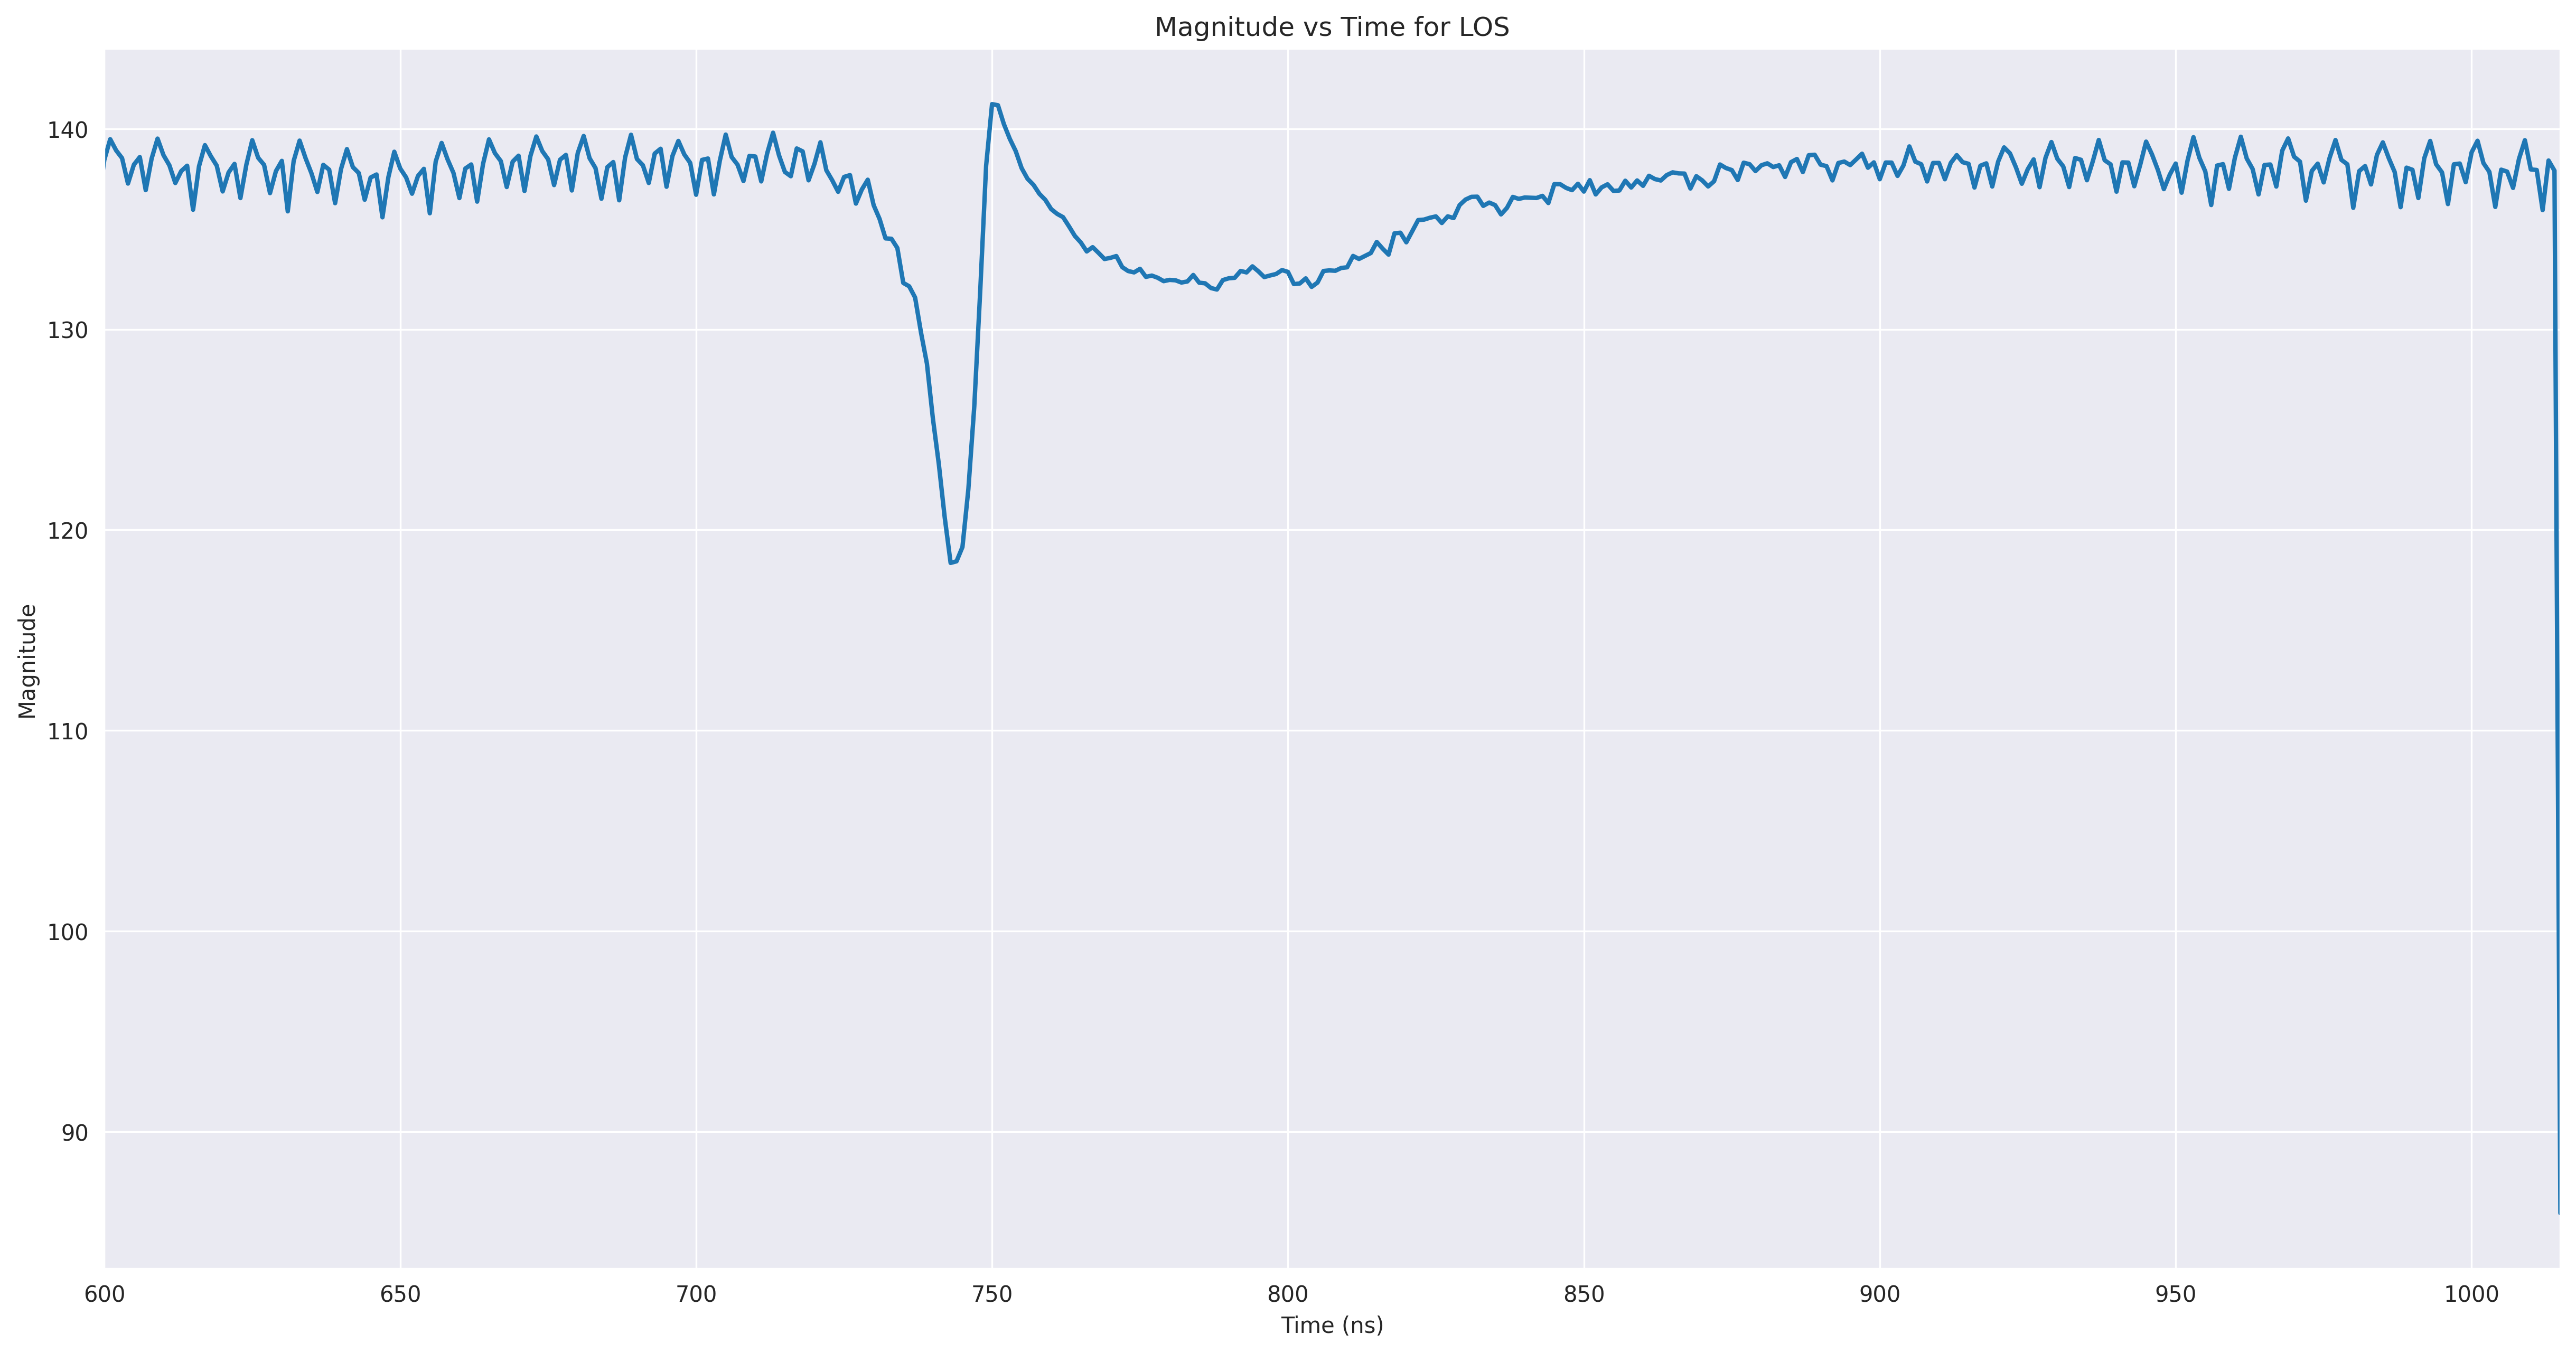
\includegraphics[width=1\textwidth]{preprocessing/lr_denoise_LOS_Scaled.png}
  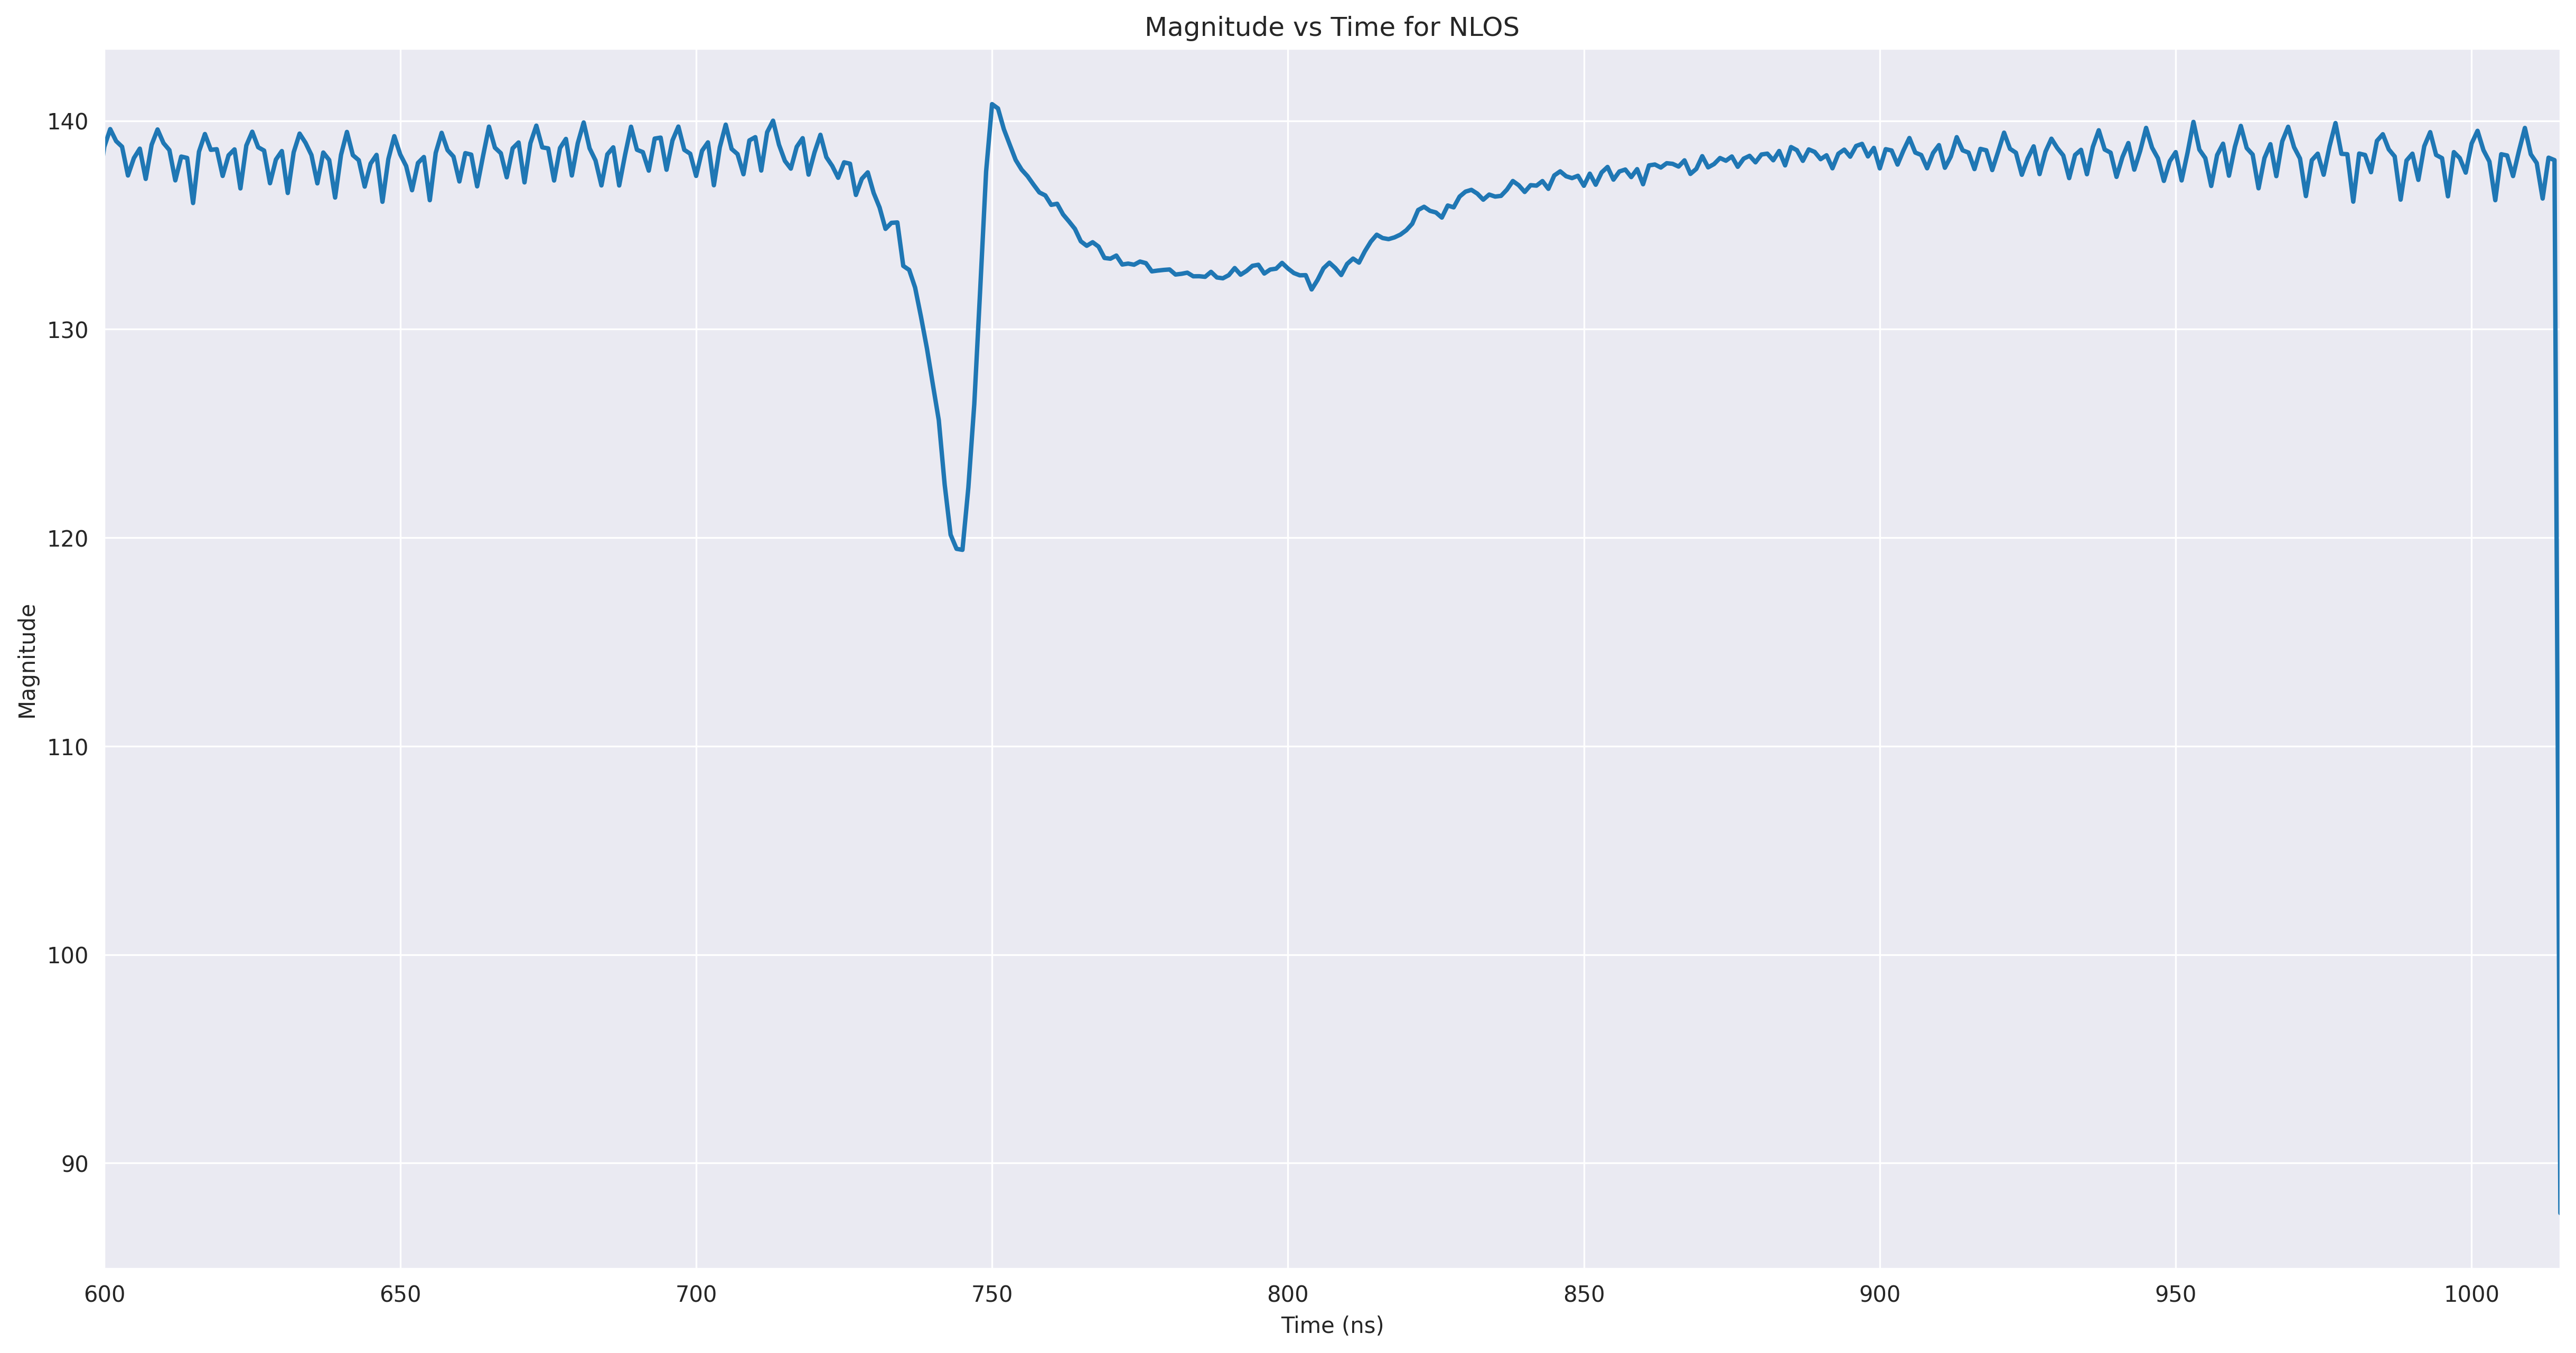
\includegraphics[width=1\textwidth]{preprocessing/lr_denoise_NLOS_Scaled.png}
  \caption{Frequency Graph of Lucy-Richardson(scaled) LOS and NLOS}\label{fig:frequency_graph_lr_scaled}
\end{figure}

\subsubsection{Signal to Noise Ratio}\label{sur_visual}

\begin{figure}[H] % [H] forces the figure to be placed exactly where it appears in the text
	\centering % Horizontally center the figure
	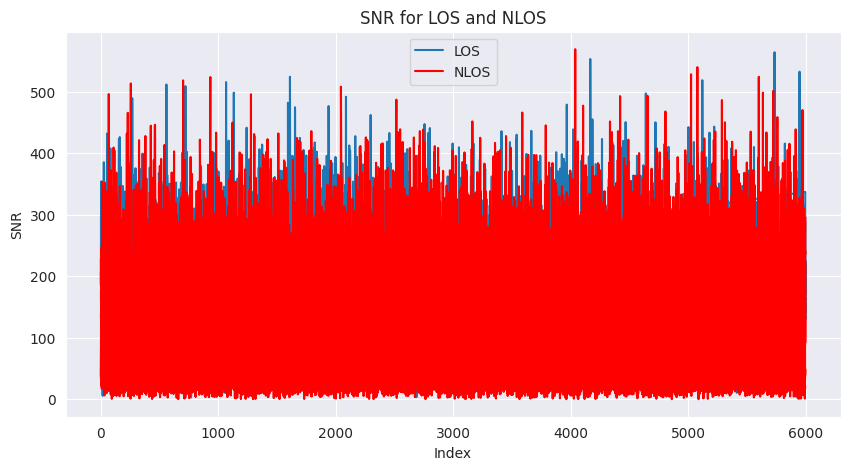
\includegraphics[width=1\textwidth]{preprocessing/SNR} % Include the figure
	\caption{Signal to Noise Ratio}\label{fig:snr}
\end{figure}


\subsection{Convolution Neural Network}\label{cnn_visual}

\begin{figure}[H] 
  \centering
  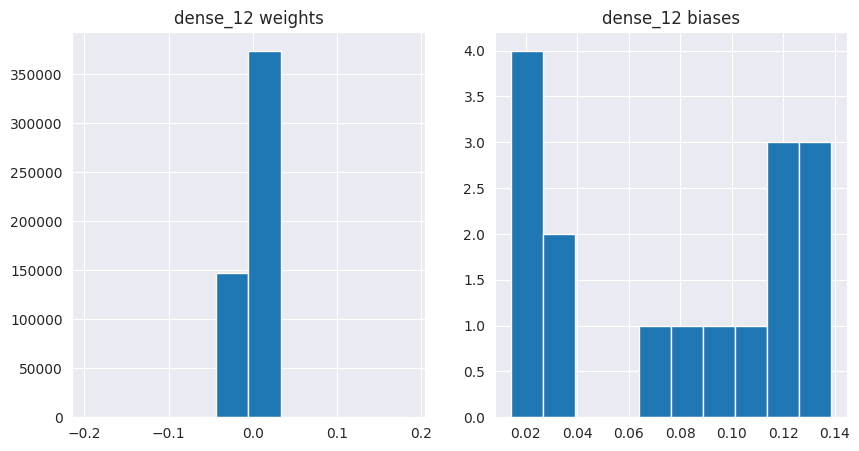
\includegraphics[width=1\textwidth]{cnn/CNN_Weight_Bias1.png}
  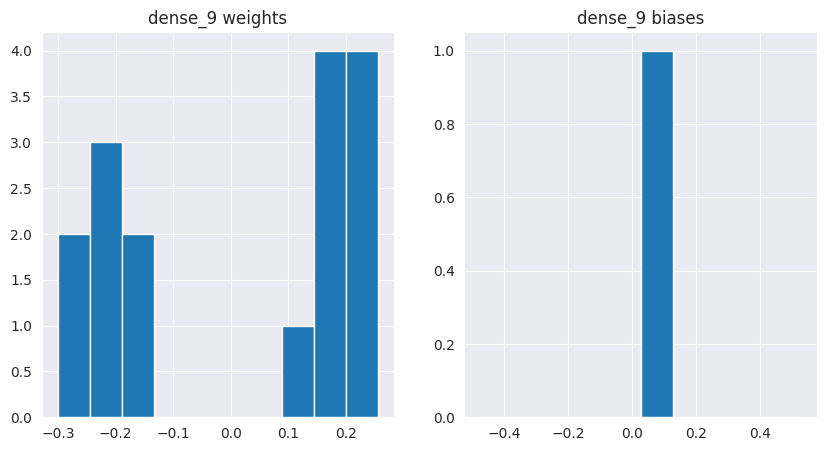
\includegraphics[width=1\textwidth]{cnn/CNN_Weight_Bias2.png}
  \caption{CNN Weights and Biases Evaluation}\label{fig:cnn_weight_bias}
\end{figure}

\begin{figure}[H] 
  \centering
  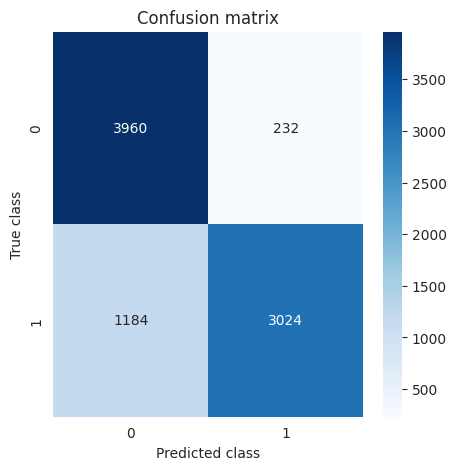
\includegraphics[width=1\textwidth]{cnn/CNN_Confusion_Matrix.png}
  \caption{CNN Confusion Matrix}\label{fig:cnn_confusion_matrix}
\end{figure}

\begin{figure}[H] 
  \centering
  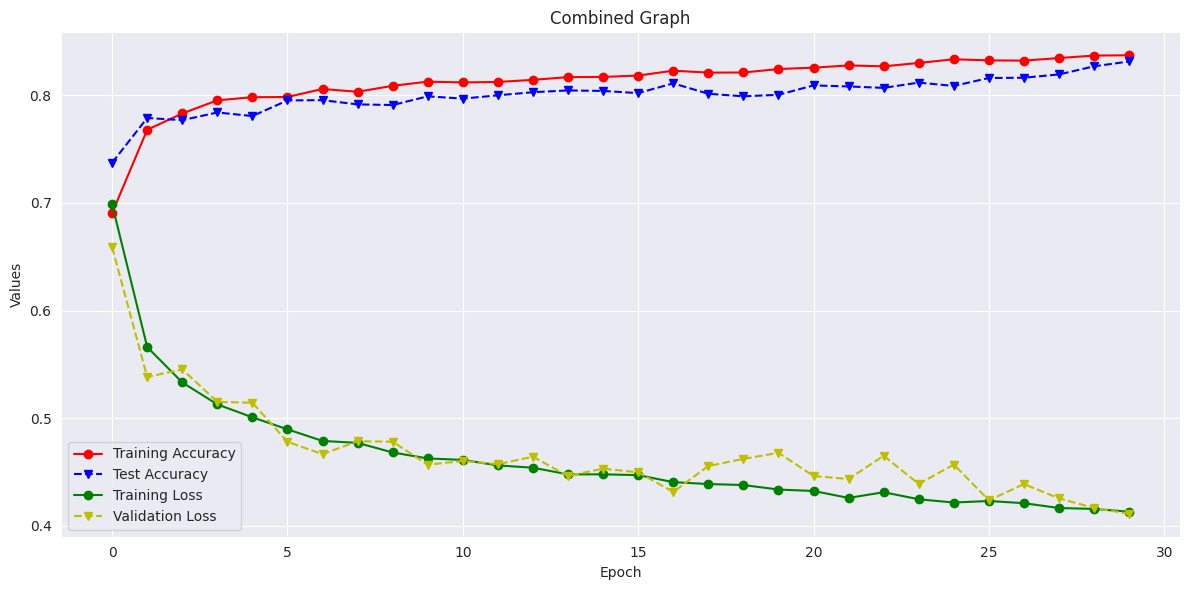
\includegraphics[width=1\textwidth]{cnn/CNN_Learning_Curve.png}
  \caption{CNN Learning Curve}\label{fig:cnn_learning_curve}
\end{figure}

\subsection{Multilayer Perceptron}\label{mlp_visual}

\subsubsection{Weights and Biases Evaluation}\label{mlp_weights_biases}

\begin{figure}[H] 
  \centering
  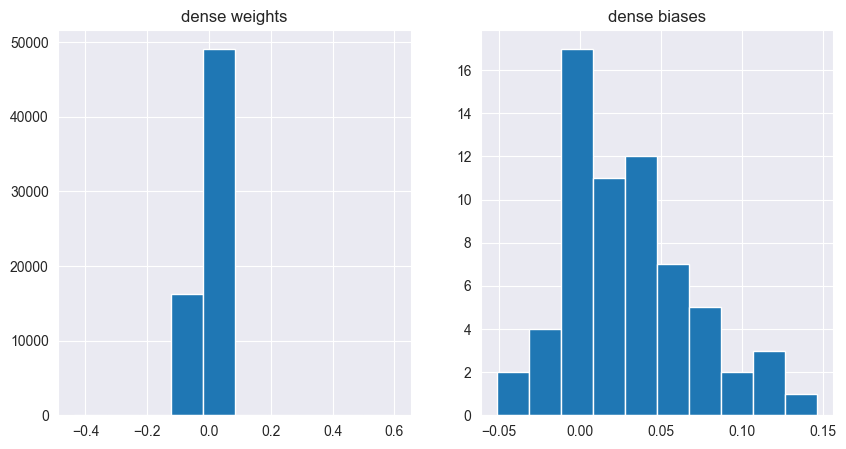
\includegraphics[width=1\textwidth]{mlp/Mlp_dense_biases.png}
  \caption{Weights and Biases Evaluation}\label{fig:mlp_weights_biases}
\end{figure}

\begin{figure}[H] 
  \centering
  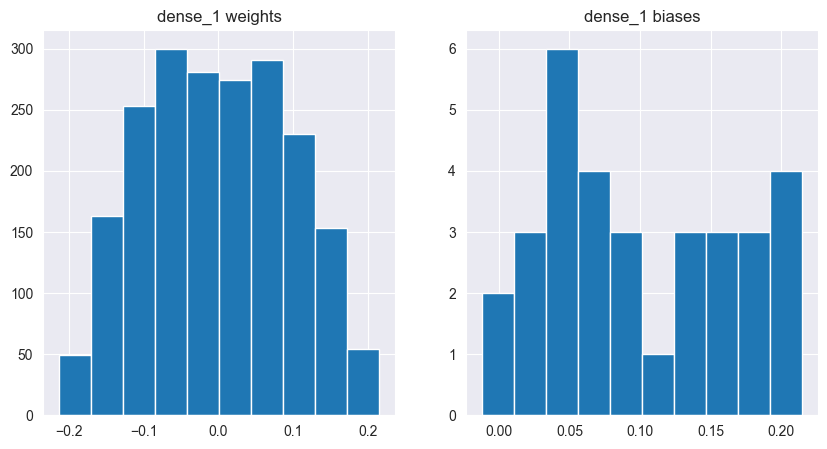
\includegraphics[width=1\textwidth]{mlp/Mlp_dense1_bias1.png}
  \caption{Weights and Biases Evaluation}\label{fig:dense1_bias1}
\end{figure}

\begin{figure}[H] 
  \centering
  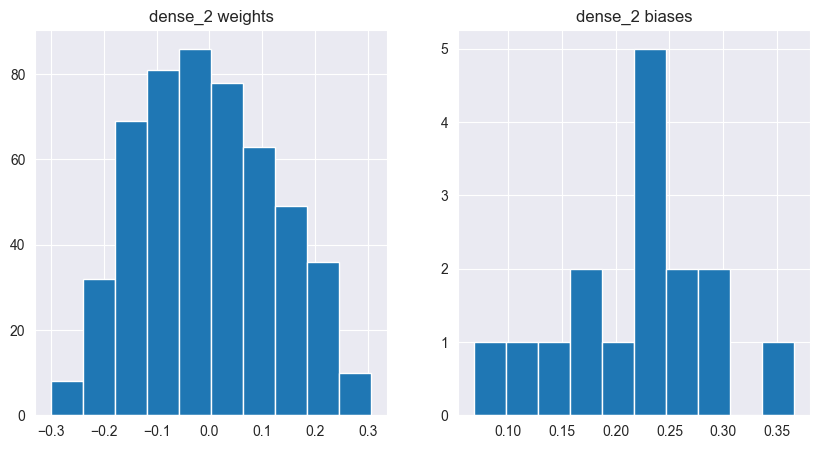
\includegraphics[width=1\textwidth]{mlp/Mlp_dense2_bias2.png}
  \caption{Weights and Biases Evaluation}\label{fig:dense2_bias2}
\end{figure}

\begin{figure}[H] 
  \centering
  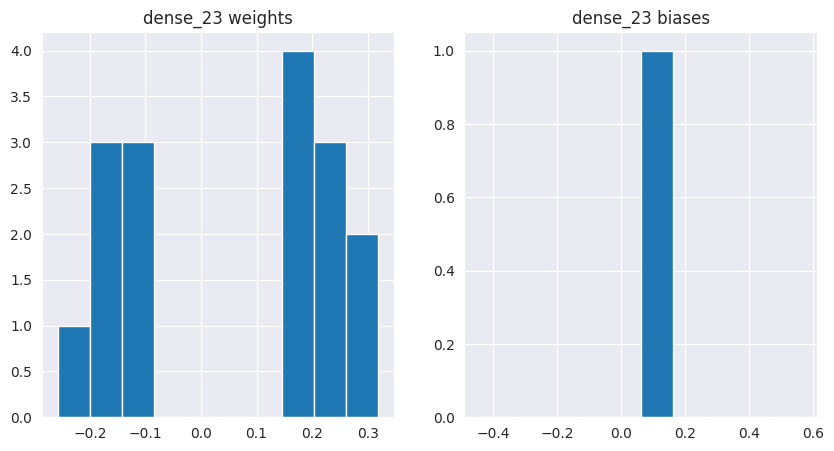
\includegraphics[width=1\textwidth]{mlp/Mlp_dense3_bias3.png}
  \caption{Weights and Biases Evaluation}\label{fig:dense3_bias3}
\end{figure}

\begin{figure}[H] 
  \centering
  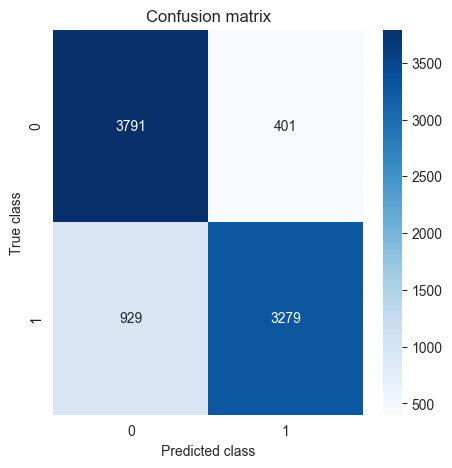
\includegraphics[width=1\textwidth]{mlp/Mlp_confusion_matrix.png}
  \caption{Confusion Matrix Evaluation}\label{fig:mpl_confusion_matrix}
\end{figure}

\begin{figure}[H] 
  \centering
  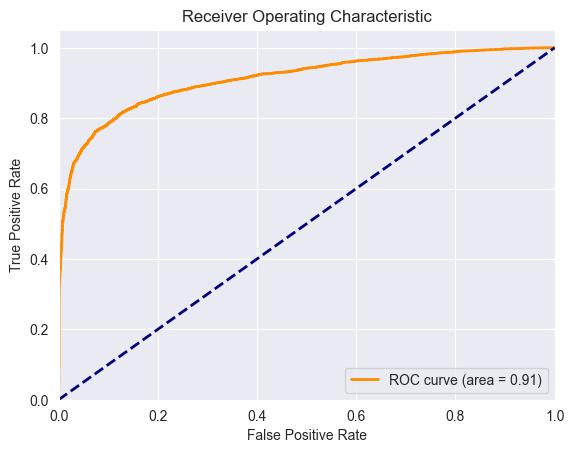
\includegraphics[width=1\textwidth]{mlp/Mlp_ROC_Curve.png}
  \caption{ROC Curve Evaluation}\label{fig:mpl_roc_curve}
\end{figure}
